\section{\mdl}
\mdl is an extension of \sdl that, in addition to defining behavior for concurrency across clients, introduces the capability for concurrency per clients. Clients are front-end applications, running on webservers, that submit requests to stateful services, such as databases or kv-stores, running on storage servers located within the same datacenter or different datacenters as the webservers.

Existing protocols that provide \sdl assume clients abide by the restriction to single-dispatch requests, having at most one outstanding request at a time. This assumption comes from the definition of linearizability, which requires individual clients to behave sequentially. These protocols, such as Paxos, Raft, Viewstamped Replication, Zab, do not provide any guarantees on the order that concurrent requests issued from a single client take effect. Our definition of \md specifies that concurrent requests issued from a single client take effect in invocation order. 

\begin{figure}[!htb]
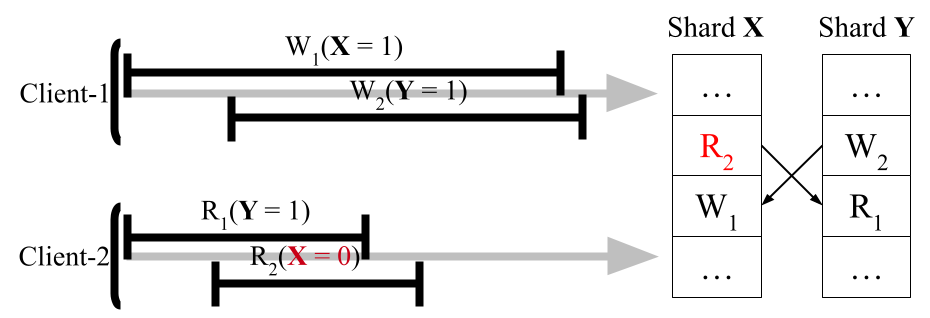
\includegraphics[scale=.45]{somet.png}
\caption{Example execution where two concurrent clients each submit 2 concurrent requests. Assume keys \textbf{X} and \textbf{Y} are at different shards. It is possible that $R_2$ arrives before $W_1$ at shard \textbf{X}, and $W_2$ arrives before $R_1$ at shard \textbf{Y}. Since clients expect their concurrent requests to take affect in invocation order, if $R_1$ returns 1, then $W_1$ must have taken affect before $R_1$, so $R_2$ should necessarily return a value of 1.}
\label{fig:concurrentbatches}
\end{figure}

\begin{figure}[!htb]
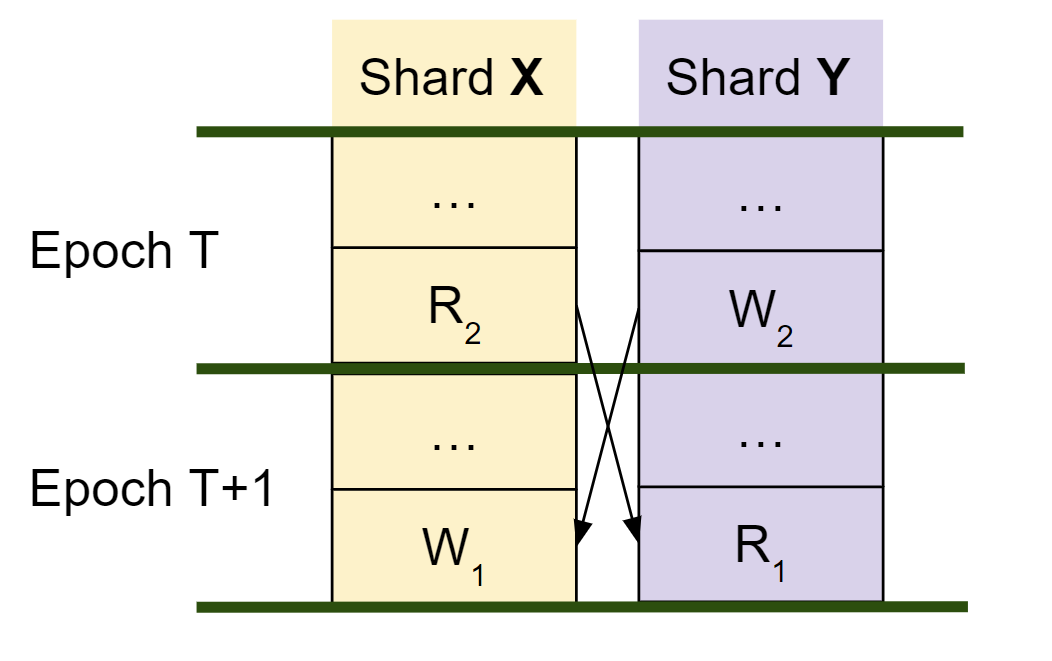
\includegraphics[scale=.3]{sorted_batching_wrong.png}
\caption{Example execution of sorted batching without coordination requirement. This execution leads to an incorrect execution that contains a cycle and is not \mdl. The execution is the same execution as that of figure \ref{fig:concurrentbatches}, but now the second request issued by each client arrives in an earlier epoch. Even if sorted in their respective epochs, they are not ordered across epochs without coordination.}
\label{fig:sortedbatchingwrong}
\end{figure}

For the single-shard setting, existing protocols come close to providing \mdl. A simple mechanism, such as per-client sequence numbers, can provide enough information for a shard leader to support invocation order for multiple requests from a single client. Such a solution does not suffice in the multi-shard setting, however, as shown in figure ~\ref{fig:concurrentbatches}. \sdl is a local property, thus a single-shard protocol correctly scales to multiple shards.  \mdl, however, is not a local property due to the possible interleaving of sets of concurrent requests across concurrent clients. This requires an \md protocol to use inter-shard communication in order to guarantee a safe total ordering that reflects issue order.
